\documentclass[journal,12pt,twocolumn]{IEEEtran}

\usepackage{setspace}
\usepackage{gensymb}
\singlespacing
\usepackage[cmex10]{amsmath}

\usepackage{amsthm}

\usepackage{mathrsfs}
\usepackage{txfonts}
\usepackage{stfloats}
\usepackage{bm}
\usepackage{cite}
\usepackage{cases}
\usepackage{subfig}

\usepackage{longtable}
\usepackage{multirow}

\usepackage{enumitem}
\usepackage{mathtools}
\usepackage{steinmetz}
\usepackage{tikz}
\usepackage{circuitikz}
\usepackage{verbatim}
\usepackage{tfrupee}
\usepackage[breaklinks=true]{hyperref}
\usepackage{graphicx}
\usepackage{tkz-euclide}

\usetikzlibrary{calc,math}
\usepackage{listings}
    \usepackage{color}                                            %%
    \usepackage{array}                                            %%
    \usepackage{longtable}                                        %%
    \usepackage{calc}                                             %%
    \usepackage{multirow}                                         %%
    \usepackage{hhline}                                           %%
    \usepackage{ifthen}                                           %%
    \usepackage{lscape}     
\usepackage{multicol}
\usepackage{chngcntr}

\DeclareMathOperator*{\Res}{Res}

\renewcommand\thesection{\arabic{section}}
\renewcommand\thesubsection{\thesection.\arabic{subsection}}
\renewcommand\thesubsubsection{\thesubsection.\arabic{subsubsection}}

\renewcommand\thesectiondis{\arabic{section}}
\renewcommand\thesubsectiondis{\thesectiondis.\arabic{subsection}}
\renewcommand\thesubsubsectiondis{\thesubsectiondis.\arabic{subsubsection}}
\newcommand*{\permcomb}[4][0mu]{{{}^{#3}\mkern#1#2_{#4}}}
\newcommand*{\perm}[1][-3mu]{\permcomb[#1]{P}}
\newcommand*{\comb}[1][-1mu]{\permcomb[#1]{C}}

\hyphenation{op-tical net-works semi-conduc-tor}
\def\inputGnumericTable{}                                 %%

\lstset{
%language=C,
frame=single, 
breaklines=true,
columns=fullflexible
}
\begin{document}

\newcommand{\BEQA}{\begin{eqnarray}}
\newcommand{\EEQA}{\end{eqnarray}}
\newcommand{\define}{\stackrel{\triangle}{=}}
\bibliographystyle{IEEEtran}
\raggedbottom
\setlength{\parindent}{0pt}
\providecommand{\mbf}{\mathbf}
\providecommand{\pr}[1]{\ensuremath{\Pr\left(#1\right)}}
\providecommand{\qfunc}[1]{\ensuremath{Q\left(#1\right)}}
\providecommand{\sbrak}[1]{\ensuremath{{}\left[#1\right]}}
\providecommand{\lsbrak}[1]{\ensuremath{{}\left[#1\right.}}
\providecommand{\rsbrak}[1]{\ensuremath{{}\left.#1\right]}}
\providecommand{\brak}[1]{\ensuremath{\left(#1\right)}}
\providecommand{\lbrak}[1]{\ensuremath{\left(#1\right.}}
\providecommand{\rbrak}[1]{\ensuremath{\left.#1\right)}}
\providecommand{\cbrak}[1]{\ensuremath{\left\{#1\right\}}}
\providecommand{\lcbrak}[1]{\ensuremath{\left\{#1\right.}}
\providecommand{\rcbrak}[1]{\ensuremath{\left.#1\right\}}}
\theoremstyle{remark}
\newtheorem{rem}{Remark}
\newcommand{\sgn}{\mathop{\mathrm{sgn}}}
\providecommand{\abs}[1]{\vert#1\vert}
\providecommand{\res}[1]{\Res\displaylimits_{#1}} 
\providecommand{\norm}[1]{\lVert#1\rVert}
%\providecommand{\norm}[1]{\lVert#1\rVert}
\providecommand{\mtx}[1]{\mathbf{#1}}
\providecommand{\mean}[1]{E[ #1 ]}
\providecommand{\fourier}{\overset{\mathcal{F}}{ \rightleftharpoons}}
%\providecommand{\hilbert}{\overset{\mathcal{H}}{ \rightleftharpoons}}
\providecommand{\system}{\overset{\mathcal{H}}{ \longleftrightarrow}}
	%\newcommand{\solution}[2]{\textbf{Solution:}{#1}}
\newcommand{\solution}{\noindent \textbf{Solution: }}
\newcommand{\cosec}{\,\text{cosec}\,}
\providecommand{\dec}[2]{\ensuremath{\overset{#1}{\underset{#2}{\gtrless}}}}
\newcommand{\myvec}[1]{\ensuremath{\begin{pmatrix}#1\end{pmatrix}}}
\newcommand{\mydet}[1]{\ensuremath{\begin{vmatrix}#1\end{vmatrix}}}
\numberwithin{equation}{subsection}
\makeatletter
\@addtoreset{figure}{problem}
\makeatother
\let\StandardTheFigure\thefigure
\let\vec\mathbf
\renewcommand{\thefigure}{\theproblem}
\def\putbox#1#2#3{\makebox[0in][l]{\makebox[#1][l]{}\raisebox{\baselineskip}[0in][0in]{\raisebox{#2}[0in][0in]{#3}}}}
     \def\rightbox#1{\makebox[0in][r]{#1}}
     \def\centbox#1{\makebox[0in]{#1}}
     \def\topbox#1{\raisebox{-\baselineskip}[0in][0in]{#1}}
     \def\midbox#1{\raisebox{-0.5\baselineskip}[0in][0in]{#1}}
\vspace{3cm}
\title{AI1103-Assignment 2}
\author{ SIRI CHANDRA-MS20BTECH11025}
\maketitle
\newpage
\bigskip
\renewcommand{\thefigure}{\theenumi}
\renewcommand{\thetable}{\theenumi}
Download all python codes from 
\begin{lstlisting}
https://github.com/siri003/AI1103-PROBABILITY-AND-RANDOM-VARIABLES/blob/main/Assignment_2/Assignment_2.py
\end{lstlisting}
%
and latex codes from 
%
\begin{lstlisting}
https://github.com/siri003/AI1103-PROBABILITY-AND-RANDOM-VARIABLES/blob/main/Assignment_2/Assignment_2.tex
\end{lstlisting}
\textbf{Problem Statement:} A and B are friends. They decide to meet between 1PM and 2PM on a given day. There is a condition that whoever arrives first will not wait for the other more than 15 minutes . The probability that they will meet on that day is \newline
\\
$(A)\frac{1}{4} \quad (B)\frac{1}{16} \quad (C)\frac{7}{16} \quad (D)\frac{9}{16}$ 
\\
\textbf{Solution:}
\\
Let A arrive at x minutes after 1PM.
\\
Let B arrive at y minutes after 1PM.
\\
The condition on x and y is 
\begin{align}
    x,y \in [0,60]
    \label{eq:eq1}
\end{align}
\begin{enumerate}
    \item 
    If A and B should meet on that day then they should satisfy the following condition along with the above condition
\begin{align}
    \abs {x-y}\leq{15}
    \label{eq:eq2}
\end{align}    
\begin{figure}[ht]
    \centering
    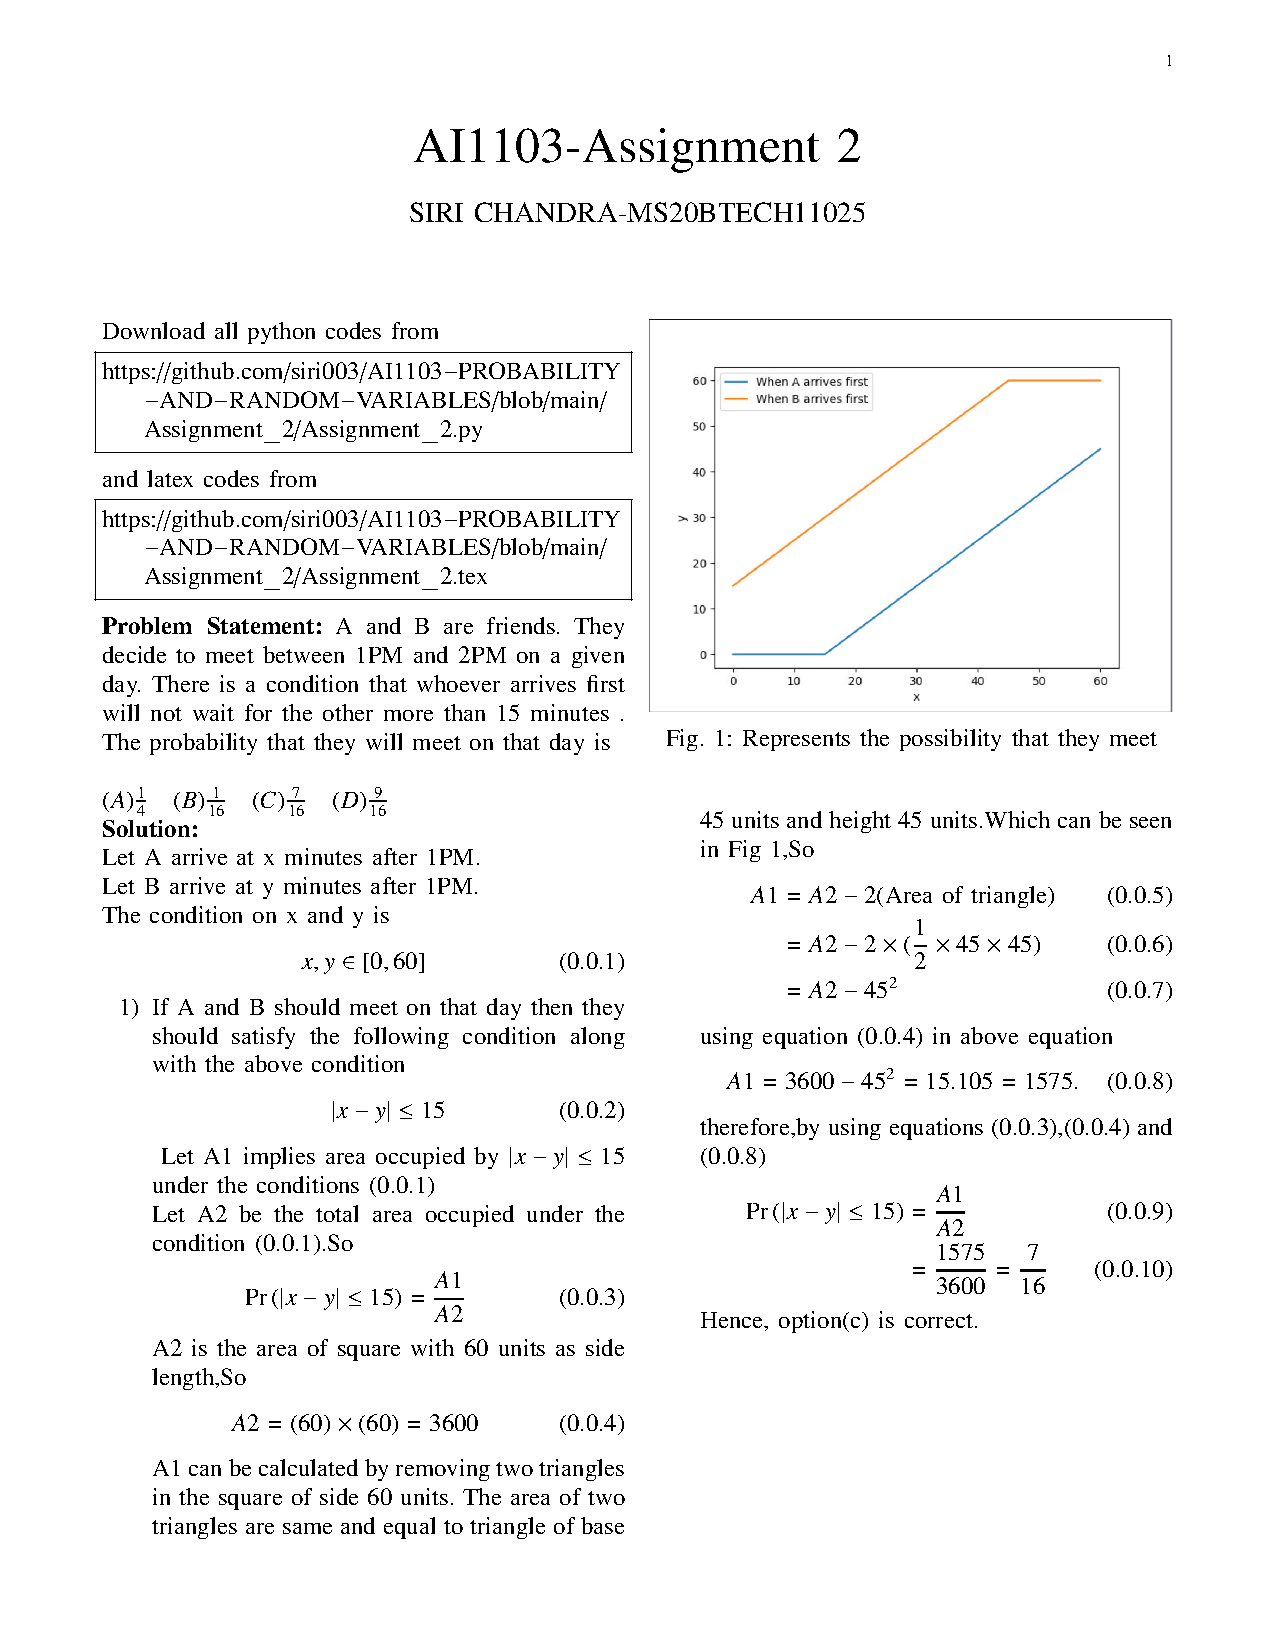
\includegraphics[width=\columnwidth]{Assignment_2.png}
    \caption{Represents the possibility that  they meet }
    \label{fig:graph1}
\end{figure}
Let A1 implies area occupied by $\abs{x-y}\leq 15 $ under the conditions \eqref{eq:eq1}
\\
Let A2 be the total area occupied under the condition \eqref{eq:eq1}.So
\begin{align}
    \pr{\abs{x - y}\leq15}&=\frac{A1}{A2}
    \label{eq:eq3}
\end{align}
A2 is the area of square with 60 units as side length,So
\begin{align}
    A2&=(60)\times(60)=3600
    \label{eq:eq4}
\end{align}
A1 can be calculated by removing two triangles in the square of side 60 units. The area of two triangles are same and equal to 
triangle of base 45 units and height 45 units.Which can be seen in Fig \ref{fig:graph1},So
\begin{align}
    A1&=A2-2(\text{Area of triangle})
    \\
    &=A2-2\times(\frac{1}{2}\times45\times45)
    \\
    &=A2 -45^{2}
    \label{eq:eq5}
\end{align}
using equation \eqref{eq:eq4} in above equation
\begin{align}
    A1&=3600-45^{2}=15.105=1575 .
    \label{eq:eq6}
\end{align}
therefore,by using equations \eqref{eq:eq3},\eqref{eq:eq4} and \eqref{eq:eq6}
\begin{align}
    \pr{\abs{x - y}\leq15}&=\frac{A1}{A2}
    \\
    &=\frac{1575}{3600}=\frac{7}{16}
\end{align}
 Hence, option(c) is correct.
\end{enumerate}

\end{document}
